% Samostalna slika: arhitektura serverske strane
% Prevesti sa:  pdflatex slika-server.tex
% Ubaciti u rad sa: 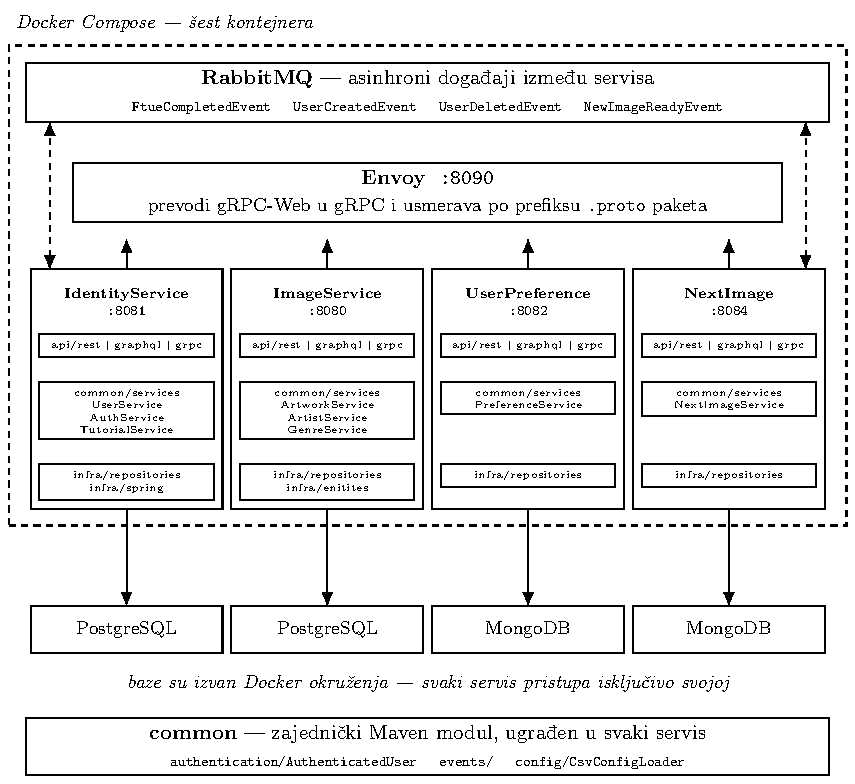
\includegraphics[width=\textwidth]{slika-server}
\documentclass[border=4pt]{standalone}
\usepackage[T1]{fontenc}
\usepackage[utf8]{inputenc}
\usepackage[english,serbian]{babel}
\usepackage{tikz}
\usetikzlibrary{arrows.meta,positioning,fit,backgrounds}

\tikzset{
  kutija/.style={draw=black,line width=0.5pt,align=center,inner sep=3pt},
  unutra/.style={kutija,minimum width=2.95cm,font=\tiny},
  servis/.style={kutija,minimum width=3.25cm,minimum height=4.05cm},
  baza/.style={kutija,minimum width=3.25cm,minimum height=0.8cm,font=\small},
  str/.style={-{Latex[length=2.2mm,width=1.8mm]},line width=0.5pt,black},
  strd/.style={-{Latex[length=2.2mm,width=1.8mm]},line width=0.5pt,black,dashed},
  strdd/.style={{Latex[length=2.2mm,width=1.8mm]}-{Latex[length=2.2mm,width=1.8mm]},
                line width=0.5pt,black,dashed},
}

\begin{document}
\begin{tikzpicture}

  % ---------- RABBITMQ (najgore, van putanje strelica ka bazama) ----------
  \node[kutija,minimum width=13.6cm,minimum height=1.0cm,anchor=north] (mq) at (0,0)
       {\textbf{RabbitMQ} --- asinhroni događaji između servisa\\[1pt]
        \scriptsize\texttt{FtueCompletedEvent} \quad \texttt{UserCreatedEvent} \quad
        \texttt{UserDeletedEvent} \quad \texttt{NewImageReadyEvent}};

  % ---------- ENVOY ----------
  \node[kutija,minimum width=12.0cm,minimum height=1.0cm,anchor=north] (envoy) at (0,-1.7)
       {\textbf{Envoy} \ \texttt{:8090}\\[1pt]
        \small prevodi gRPC-Web u gRPC i usmerava po prefiksu \texttt{.proto} paketa};

  % ---------- SERVISI ----------
  \foreach \x/\ime/\port/\srv/\inf in {%
      -5.1/IdentityService/8081/{UserService\\AuthService\\TutorialService}/{infra/repositories\\infra/spring},
      -1.7/ImageService/8080/{ArtworkService\\ArtistService\\GenreService}/{infra/repositories\\infra/enitites},
       1.7/UserPreference/8082/{PreferenceService}/{infra/repositories},
       5.1/NextImage/8084/{NextImageService}/{infra/repositories}}
  {
    \node[servis,anchor=north] (s\ime) at (\x,-3.5) {};
    \node[anchor=north,font=\scriptsize,align=center] at ([yshift=-2mm]s\ime.north)
         {\textbf{\ime}\\\texttt{:\port}};
    \node[unutra,anchor=north] at ([yshift=-11mm]s\ime.north)
         {api/rest \textbar{} graphql \textbar{} grpc};
    \node[unutra,anchor=north] at ([yshift=-19mm]s\ime.north)
         {common/services\\\srv};
    \node[unutra,anchor=north] at ([yshift=-33mm]s\ime.north)
         {\inf};
    \draw[str] (s\ime.north) -- ++(0,0.5);
  }

  % dogadjaji: uspravne trake pored Envoy-a, u oba smera (objava i prijem)
  \draw[strdd] (-6.4,-3.5) -- ([xshift=-64mm]mq.south);
  \draw[strdd] ( 6.4,-3.5) -- ([xshift=64mm]mq.south);

  % ---------- DOCKER GRANICA ----------
  \begin{scope}[on background layer]
    \node[draw=black,line width=0.7pt,dashed,inner sep=8pt,
          fit=(mq)(envoy)(sIdentityService)(sNextImage)] (docker) {};
  \end{scope}
  \node[anchor=south west,font=\small\itshape] at ([yshift=1mm]docker.north west)
       {Docker Compose --- šest kontejnera};

  % ---------- BAZE (izvan Docker-a) ----------
  \node[baza,anchor=north] (db1) at (-5.1,-9.2) {PostgreSQL};
  \node[baza,anchor=north] (db2) at (-1.7,-9.2) {PostgreSQL};
  \node[baza,anchor=north] (db3) at ( 1.7,-9.2) {MongoDB};
  \node[baza,anchor=north] (db4) at ( 5.1,-9.2) {MongoDB};

  \draw[str] (sIdentityService.south) -- (db1.north);
  \draw[str] (sImageService.south)    -- (db2.north);
  \draw[str] (sUserPreference.south)  -- (db3.north);
  \draw[str] (sNextImage.south)       -- (db4.north);

  \node[font=\small\itshape,anchor=north] at (0,-10.25)
       {baze su izvan Docker okruženja --- svaki servis pristupa isključivo svojoj};

  % ---------- COMMON ----------
  \node[kutija,minimum width=13.6cm,minimum height=0.85cm,anchor=north]
       (common) at (0,-11.1)
       {\textbf{common} --- zajednički Maven modul, ugrađen u svaki servis\\[1pt]
        \scriptsize\texttt{authentication/AuthenticatedUser} \quad \texttt{events/}
        \quad \texttt{config/CsvConfigLoader}};

\end{tikzpicture}
\end{document}
